%------------------------------------------------------------------------
%  交通流のシミュレーション 
%  The Mathematical Society of Traffic Flow
%  
%  Ver. 1.0 05/12/09  H. Watanabe
%------------------------------------------------------------------------

\documentclass[twocolumn]{jarticle} %二段組の場合
%\documentclass[onecolumn]{jarticle}  %一段組の場合

\usepackage{mstf2}
\usepackage[dvipdfmx]{graphicx}
\usepackage{graphicx}
\usepackage{mathtools}
\graphicspath{{./pic/}}
\usepackage{gensymb}
%------------------------------------------------------------------------

%------------------------------------------------------------------------
%コンパイルコマンド
%1. platex thesis.tex
%2. platex thesis.tex
%3. dvipdfmx thesis.dvi
%4. evince thesis.pdf &
%------------------------------------------------------------------------


\title{%和文タイトル
非線形感覚運動写像ロボットの不完全対面流\\
{\Large -1方向走行流への転移と流量のコース幅依存性-}
}

\titleE{%英文タイトル
Incomplete robots counter flow based on Non-linear sensory motor mapping\\
{\Large -Transition to one-way flow and relations between course and flow rate-}
}

\author{%和文氏名
李 方正$^1$, 橋爪 晋平$^2$,本田 泰$^3$
}

\authorE{%英文氏名
Li Fangzheng$^1$, Shimpei Hashizume $^2$,Yasushi Honda $^3$
}

\affiliation{%和文所属
$^1$ 室蘭工業大学大学院 工学研究科 情報電子工学系専攻\\
$^2$ 室蘭工業大学 工学部 情報電子工学系学科\\
$^3$ 室蘭工業大学大学院 しくみ解明系領域
}

\affiliationE{%英文所属
$^1$ Division of Information and Electronic 
Engineering, Graduate School of Engineering, Muroran Institute of Technology, Japan\\
$^2$ Department Information and Electronic 
Engineering,  School of Engineering, Muroran Institute of Technology, Japan\\
$^3$ College of Information and Systems, Muroran Institute of Technology, Japan
}

\abst{%和文概要
本研究では,昆虫や人間の対面走行行為にどんな知能を持っているかを解明するため,ラズパイを基づいてtof距離センサー3つ搭載され,ハイパボリックタンジェント(tanh)関数でセンサーからもらった距離デーダーをロボットの左右モーターの出力に写像して,障害物を避ける走行ロボット開発した.そのロボットを使って,楕円コースで異なる台数のロボットの対面走行実験をして,ロボットの時速,流量とone direction flowになるまでの時間を測定した.結果として,時間とともに,どんな初期配置でも,結局,全てのロボットが同じ向きで走り(one direction flow)になる傾向があると観測した.one direction flow になる時間が幅の拡大に従って,減少していく.流量が山登りみたいに増加して幅が49.5$cm$から減少していくとわかった.
}

\abstE{%英文概要
In this research, in order to unriddle what kinds of intelligence they have in face-to-face moving of insects and humans, we developed wheeled robot which can avoid obstacles based on Raspberry Pi and we use hyperbolic tangent function to transform distance data which got by three laser sensors to of both sides of motors'power output. Then we have done some face-to-face moving experiments with different numbers'robots on ellipical course and we also measured the speed, flow rate and the time spent of robots change to the same direction.As the result,we observed that all robots tended to moving in the same direction(one direction flow)regardless of initial configuration.And we found that the time of become one direction flow increases with the increase of width and the flow rate increases first and decreases from 49.5cm.

}

%------------------------------------------------------------------------
% ここから本文
%------------------------------------------------------------------------

\begin{document}
\maketitle

\section{はじめに}
実世界で,蜂,アリなどの昆虫が簡単な振舞いや匂いで複雑な群れ行為ができる.大きな交差点で,人の密度が高いでも,皆は会話なくて,ぶつからないようにスムーズに対面走行ができる.その中に一体どんな知能が持っている,どのぐらいの知能が必要だと知りたいので,我々は原生生物レベルの感覚と運動直接関連する感覚運動写像での障害物避ける振舞い,反応行動レベルの知能を持つ走行ロボットの対面走行を始めにその知能を解明するである.本稿では,tanh関数を使い非線形感覚運動写像をモデルとし,ラズパイを基づく障害物を避ける走行ロボットを開発した.その走行ロボット(今回,最大8台使われる)を右回りと左回り(変曲点係数bで制御する)の2つグループを分けて楕円コースでの対面走行を実験して,変曲点の係数(b)と初期配置を変化させ,ロボットの振舞いを調査して,ロボットたちの時速,同じ流れになるまでの時間と流量などロボットの基本的な走行情報を測定し,one direction flow 状態を観測した.
\section{ロボットの構造}
\subsection{ロボットの身体性}
走行ロボットの正面図と俯瞰図:
\begin{figure}[h]
    \begin{minipage}{0.48\linewidth}
        \centering
        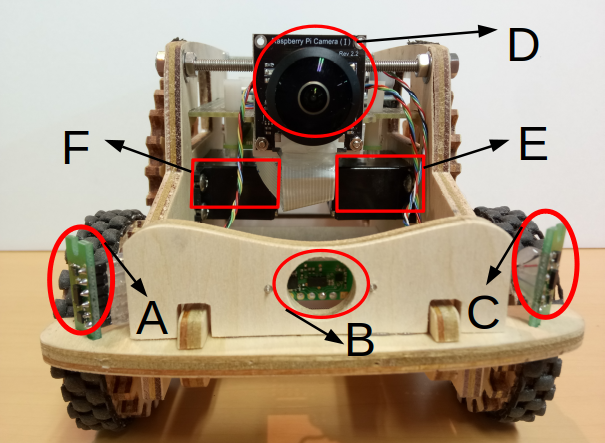
\includegraphics[width=0.9\linewidth]{robot1.jpg}
        \caption{正面図}
    \end{minipage}
    \begin{minipage}{0.48\linewidth}
        \centering
        \includegraphics[width=0.9\linewidth]{robot2.jpg}
        \caption{俯瞰図}
    \end{minipage}
\end{figure}

\begin{figure}[h]
        \centering
        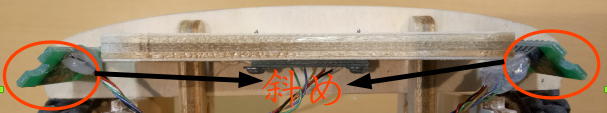
\includegraphics[width=1.0\linewidth]{robot4.jpg}
        \caption{左右のセンサー角度表示}
\end{figure}


A:右の距離センサー;B:中央の距離センサー;C:左の距離センサー;D:カメラ(使っていない);E:右モーター;F:左モーター;制御システム:ラズパイ;左右センサー角度:45\degree;ロボット幅:13.5;ロボット長さ:20.2;ロボット高さ:12.2;



今回使っているのは4輪木造走行ロボットである,人間や昆虫の走行特徴に近似するため,左右の車輪は左右のモーターで独自に制御して,超信地旋回できるようになる.tof距離センサーが赤外線の反射で距離を測るので,超音波より測る範囲が狭いけど,体積が小さく,精度が高くて,複数ロボットの場合,ロボット同士間の妨害も減少できる.

\subsection{感覚運動写像モデル}

感覚運動写像とは,センサー値を変数とする関数によってモーターの出力を決定することであり,その瞬間のセンサー値だけを使うと,最も単純な反応行動のための知能の一つである.
本研究では,非線形写像モデルが使われている.

1.距離デーダーの相乗平均:

\begin{equation}
  x_{\rm L} = e^{\gamma \ln d_{\rm C}} \cdot e^{(1-\gamma)\ln d_{\rm L}} 
\end{equation}
\begin{equation}
  x_{\rm R} = e^{\gamma \ln d_{\rm C}} \cdot e^{(1-\gamma)\ln d_{\rm R}} 
\end{equation}

中央のセンサーでもらった距離デーダー($d_{\rm C}$)と左のセンサーでもらった距離デーダー($d_{\rm L}$)が式(1)で計算して,左の感覚運動写像方程式の入力($x_{\rm L}$)がもらえる,同じように,真中のセンサーでもらった距離デーダー($d_{\rm R}$)と右のセンサーでもらった距離デーダー($d_{\rm R}$)が式(2)で計算して,右の感覚運動写像の入力($x_{\rm R}$)がもらえる.$\gamma$は重みであり,$\gamma$イコール0.33のとき,等加重である.

2.感覚運動写像:
\begin{equation}
\begin{aligned}
  m_{\rm R} = &\alpha_{1{\rm L}} \tanh(\beta_{1{\rm L}}(x_{\rm L} - b_{\rm L})) + \\
        &\alpha_{2{\rm L}} \tanh(\beta_{2{\rm L}}(x_{\rm L} - b_{\rm L})) + c_{\rm L}
\end{aligned}
\end{equation}

\begin{equation}
\begin{aligned}
  m_{\rm L} = &\alpha_{1{\rm R}} \tanh(\beta_{1{\rm R}}(x_{\rm R} - b_{\rm R})) + \\
        &\alpha_{2{\rm R}}\tanh(\beta_{2{\rm R}}(x_{\rm R} - b_{\rm R})) + c_{\rm R}
\end{aligned}
\end{equation}
式(1)と(2)でもらった$x_{\rm L}$と$x_{\rm R}$を式(3)と(4)に代入して,ロボットの右モーターの出力($m_{\rm R}$)と左モーターの出力($m_{\rm L}$)が計算できる.係数$\alpha$がロボットの最大速度を制御する,係数$\beta$が{\rm tanh}の傾きを制御する,係数$b$が関数の変曲点の位置を制御する,係数$c$が関数のだて軸上の位置を制御する. 
今回の実験のパラメーター:
$\alpha_{1{\rm L}}$,$\alpha_{2{\rm L}}$,$\alpha_{1{\rm R}}$,$\alpha_{2{\rm R}}$:30;
$\beta_{1{\rm L}}$と$\beta_{1{\rm R}}$:0.004;
$\beta_{2{\rm L}}$と$\beta_{2{\rm R}}$:10;
$c_{\rm L}$と$c_{\rm R}$:0;
ロボットグループ1の$b_{\rm L}$とロボットグループ2の$b_{\rm R}$:160;
ロボットグループ2の$b_{\rm L}$とロボットグループ1の$b_{\rm R}$:260;


\section{走行実験}
直線と円形両方あり,一回じゃなくて,ぐるぐる回って複数の対面走行できるように,楕円コースで実験する.コースの中(青い部分)にロボットをランダムに配置して速度0からほぼ同時にスタート,約8分間実験する.ロボットたちがtof距離センサーでコースの壁までの距離を測って,非線形感覚運動写像モデルにより走行する.半分のロボットが右回り($b_{\rm L}>b_{\rm R}$),残りのロボットが左回り($b_{\rm L}<b_{\rm R}$).コースの青い部分の中央に(黒い線)でコースの長さを測る,コースの長さ($L$)は7.32$m$,今回ロボットの台数($N$)は8台.コースの長さを固定し(線密度($\rho$)を固定する(式5)),両側の壁を広まったり,縮まったりして,コースの幅($w$)が$43cm$,$49.5cm$,$56cm$,$62.5cm$,$69cm$を変化し,実験する.

\begin{equation}
\rho = \frac{N}{L}
\end{equation}

\begin{figure}[!ht]
    \centering
    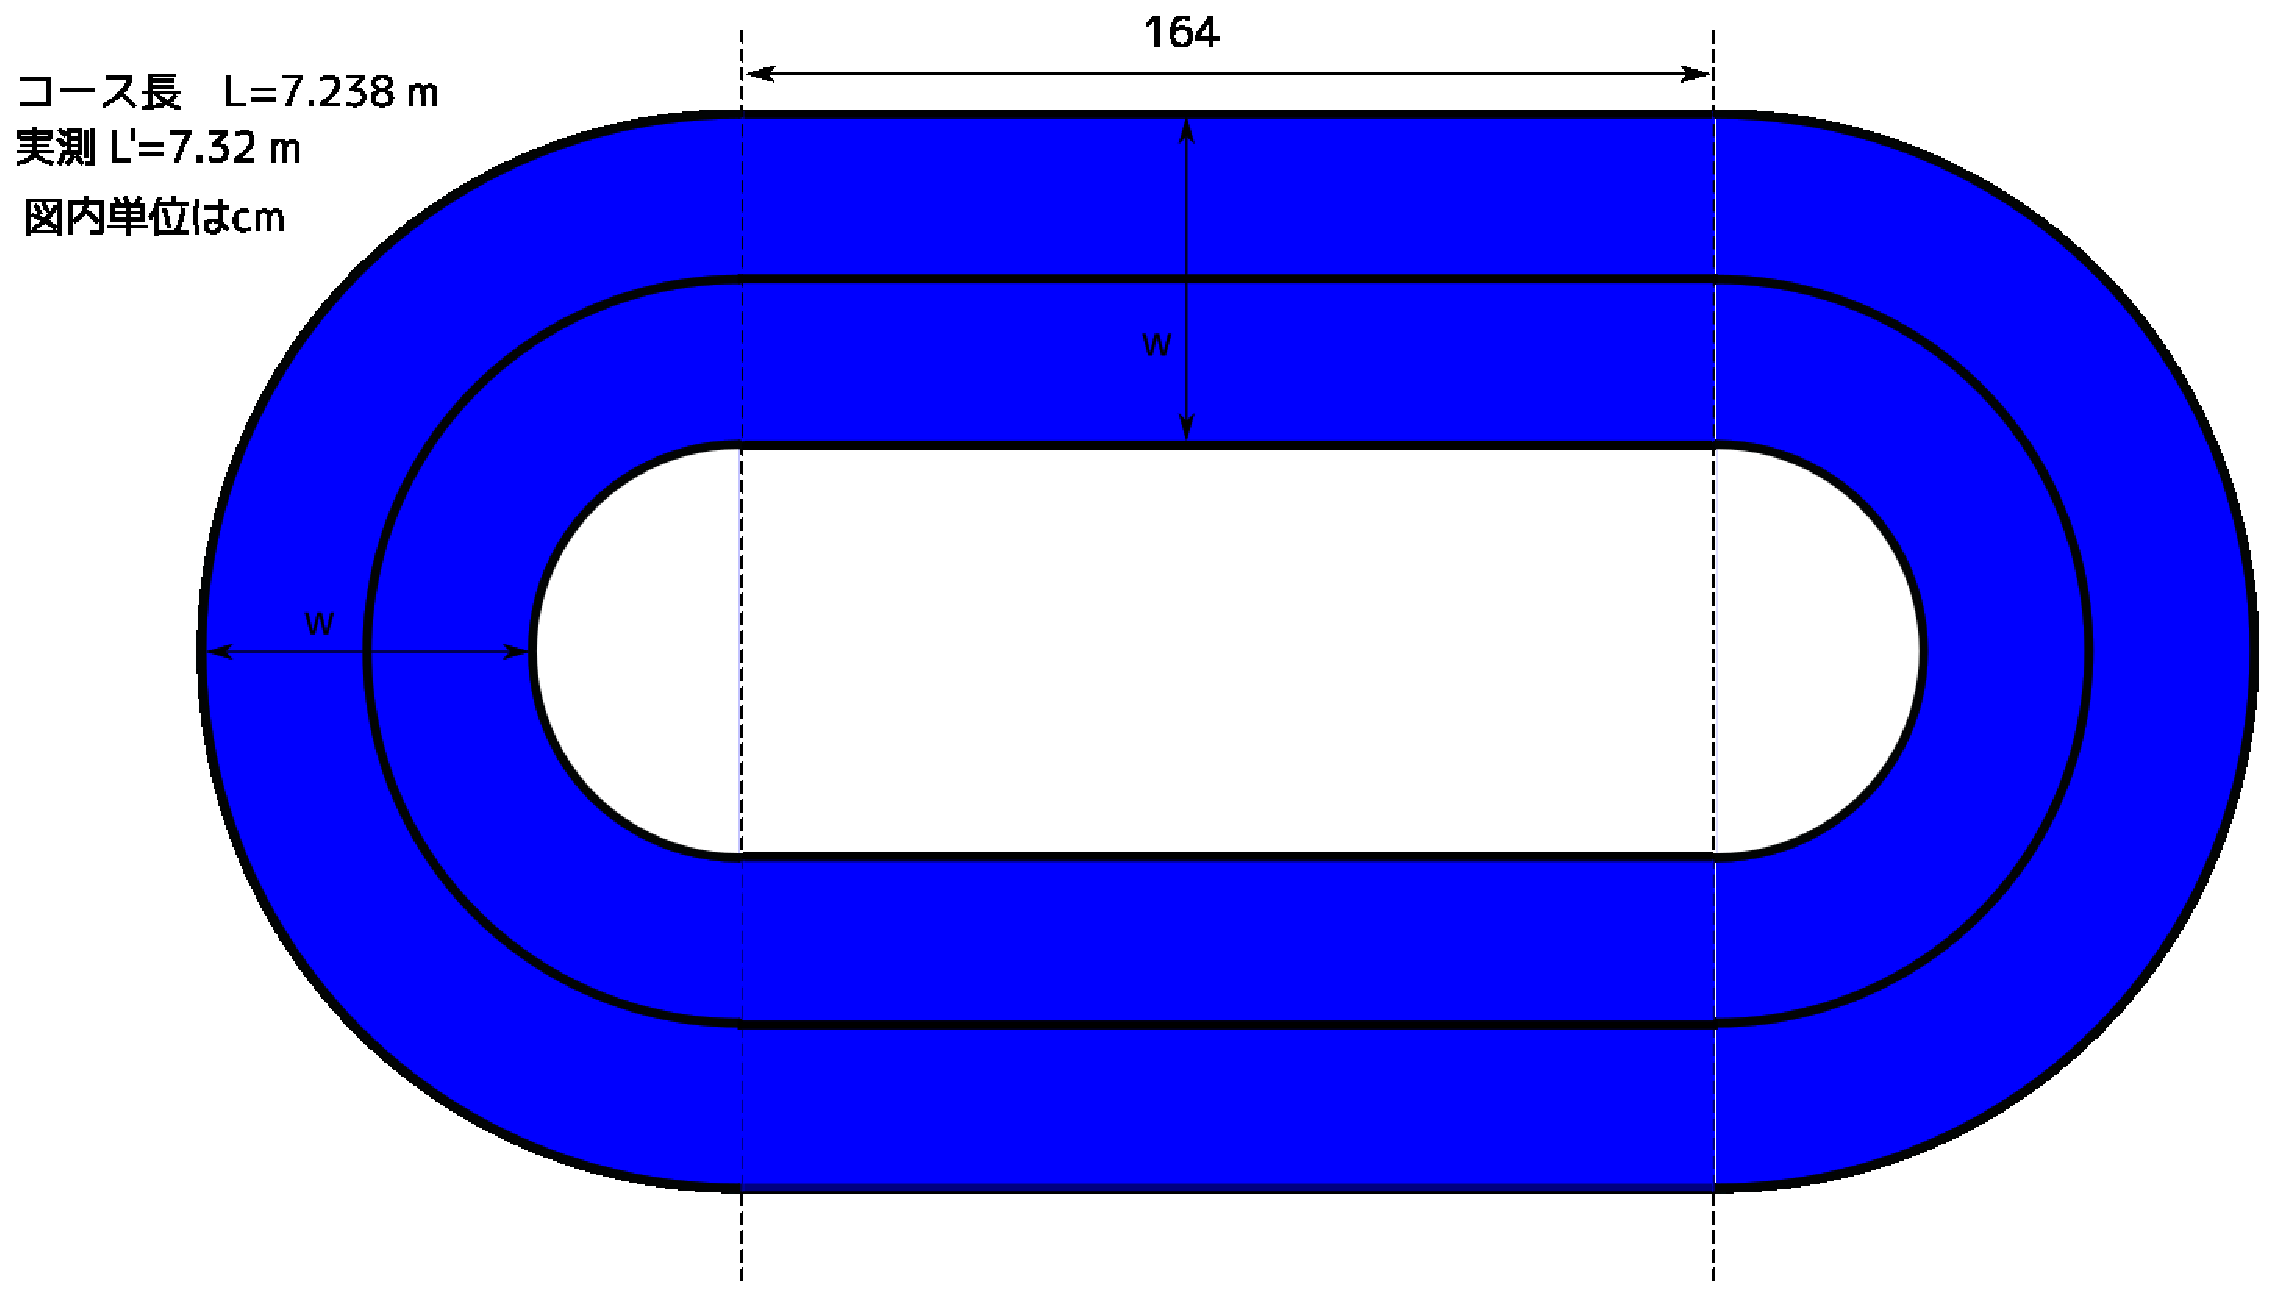
\includegraphics[width=0.7\linewidth]{Oval_h2.eps}
    \caption{コースレイアウト}
\end{figure}


\begin{figure}[h]
    \begin{minipage}{0.48\linewidth}
        \centering
        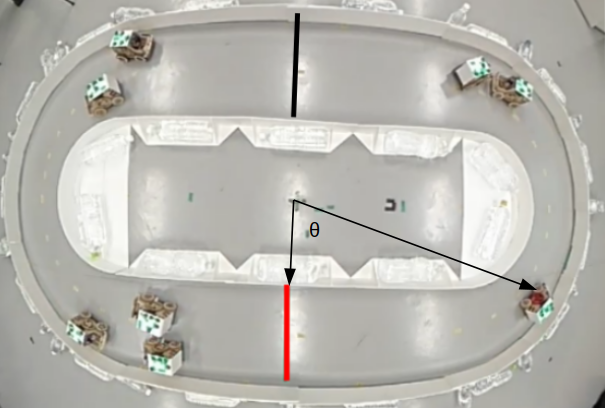
\includegraphics[width=1.0\linewidth]{course3.jpg}
        \caption{コース}
    \end{minipage}
    \begin{minipage}{0.48\linewidth}
        \centering
        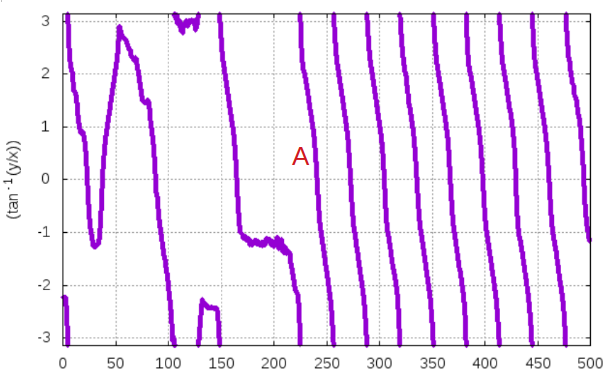
\includegraphics[width=1.0\linewidth]{number2.jpg}
        \caption{時間よりロボットの位置角度}
    \end{minipage}
\end{figure}

\begin{equation}
Q = \frac{n}{wT_{\rm sd}}
\end{equation}

図5の赤い線をベースとして,ロボットが左から右へ線を通過したら流量+1,右から左へ線を通過したら流量-1.図6の横軸が時間(0から8分間),縦軸がロボットの位置角度$\theta$(図5),ロボットが赤い線から反時計回りで黒い線まで,$\theta$が0から$\pi$に変わる.赤い線から時計回りで黒い線まで,$\theta$が0から$-\pi$に変わる.横軸の時間に従って,紫色の線が縦軸の0を交差すると,計測線(赤い線)を通過したと認めて,台数($n$)を計測する.一回の実験で図6のように図が8個あり,Aの紫色線に対応する時間が一番大きな時間がone direction flow状態(全てのロボットが同じ向きで走る$b_{\rm L}<b_{\rm R}$)になる時間($T_{\rm sd}$,単位:分)と認める.$w$がコースの幅(単位:$m$),$Q$が流量,式6で流量を計算する.


\section{実験結果}
\subsection{記号の説明}

\begin{enumerate}
\item $b_{\rm L}>b_{\rm R}$:ロボットが右曲がり易い($b_{\rm L}$の方が大きいので,同じ距離$x$で$b_{\rm L}$に対応するtanh関数の変曲点が横軸の正方向に多く移動して,$x-b_{\rm L}$が小さくなる,方程式3により,右のモーターが左のモーターより先に速度を減少するので,ロボットが右曲がりやすいである)
\item $b_{\rm L}<b_{\rm R}$:ロボットが左曲がり易い
\item 初期配置:ロボットの位置はランダムで,グループ2のロボットが左回り,グループ2のロボットが右回り.
%\item 密度:ロボット台数/コース面積
\item $T_{\rm sd}$:全てのロボットのスタートから全てのロボットが一方向走行するまでの所要時間
%\item 渋滞時間割合:$T_{\rm sd}$に対して,渋滞時間の割合
%\item 同じ流れ方向:同じ流れになる時間後の
%          一方向走行の方向
\end{enumerate}


ロボットが一つずつ5周回って,時速を計算する($v=\frac{5*L}{t}$,$v$:時速,$L$:コースの長さ,$t$:5周回る時間).時速の平均値$\bar v$:787.52$m/h$;時速の分散($s^2$):2640.3;標準偏差($s$):51.384


\subsection{幅による$T_{\rm sd}$流量の測定}
5つの幅があり,各自の幅で各十回(毎回8分間)実験する,毎回の実験で,ランダムでロボットを2つグループを分ける.$T_{\rm sd}$と流量の平均値と分散を計測する
\begin{table}[!ht]
\begin{center}
\begin{tabular}{|c|c|c|c|c|}
\hline
幅 & $T_{\rm sd}$(秒) & $T_{\rm sd}$ & 流量 & 流量 \\
($cm$)   &   平均値 & 分散 & 平均値 & 分散 \\
\hline
43 & 0 & 0 & 0 & 0 \\
\hline
49.5 & 0 & 0 & 0 & 0 \\
\hline
56 & 277.8 & 17838.56 & 2.345 & 33.558 \\
\hline
62.5 & 274.1 & 11389.69 & -0.354 & 18.399 \\
\hline
69 & 273.4 & 19343.84 & 0.118 & 41.541 \\
\hline
\end{tabular}
\end{center}
\caption{
幅により$T_{\rm sd}$と流量の値
}
\end{table}

\begin{figure}[ht]
    \centering
    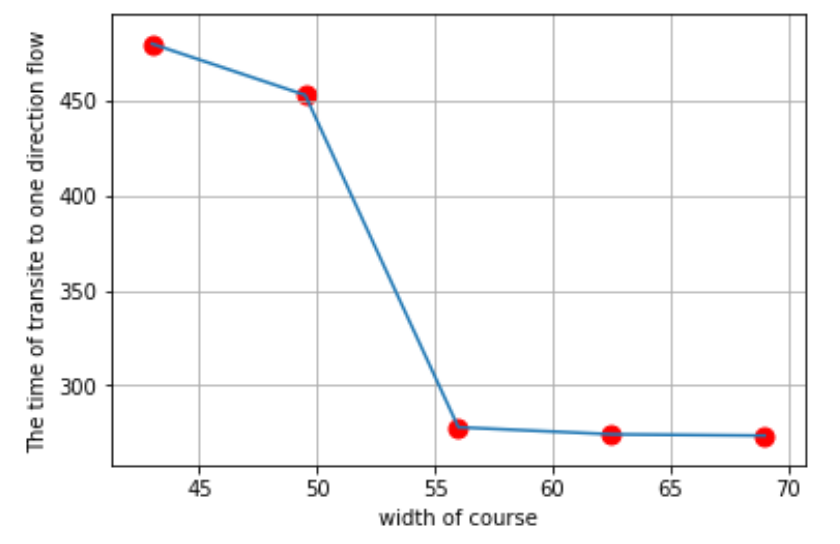
\includegraphics[width=1.0\linewidth]{diagram1.jpg}
    \caption{}
\end{figure}
\begin{figure}[ht]
    \centering
    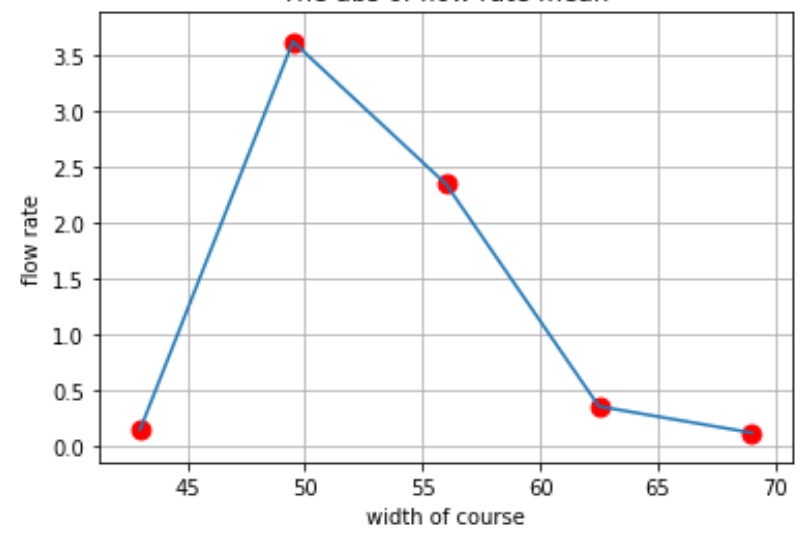
\includegraphics[width=1.0\linewidth]{diagram2.jpg}
    \caption{}
\end{figure}

図$7$が幅の拡大に従って,$T_{\rm sd}$の変化曲線である.図$8$が幅の拡大に従って,流量($Q$)の変化曲線である.
幅が狭すぎる(43$cm$)と,長時間の渋滞が発生したことを観測した,ロボット同士が互いに引っかかって,方向転換もできなくて,one direction flow の状態も出なかった.大渋滞ので,流量もほとんどない.49.5$cm$の場合,渋滞も起こったので,one direction flow 状態になる時間($T_{\rm sd}$)も長かった,ロボットがギリギリ方向転換できて,流量もふえてきた.56$cm$から渋滞がほとんどなくて,ロボットの方向転換もしやすくなって,$T_{\rm sd}$が急激に減少して,幅がもっと広まっても,あんまり変わらないようになった.それに,幅が広まっていって,右回りと左回りのロボットの数が相当で,対面走行ができて,流量も減少していった(完璧な対面走行の流量が$0$である)

\section{考察}


\end{document}




